%04chapterSelbsteinsch.tex

\chapter{Selbsteinschätzung}
In diesem Kapitel wird beschrieben, welche Rollen die Teammitglieder mittels Selbsteinsch"atzung erhalten. Dazu wird ein Test verwendet, welcher urspr"unglich von R.M. Belbin \cite{belbin1981management} entwickelt und an der Universit"at Regensburg ins Deutsche übersetzt wurde. In diesem Test werden verschiedenste Aussagen bezüglich des eigenen Verhaltens in bestimmten Situationen mittels eines Punktesystems bewertet. Am Ende trägt man die Punkte in ein Raster ein, aus welchem sich dann die passenden Rollen herauskristallisieren.

\subsection*{Pascal Horat}
Da ich in meinem Leben schon andere, ähnliche Tests ausgefüllt habe, wusste ich welche Rollen ich als Resultat in etwa zu erwarten hatte. Trotzdem war ich gespannt, ob sich auch dieses Mal dieselben Tendenzen zeigen würden. \\

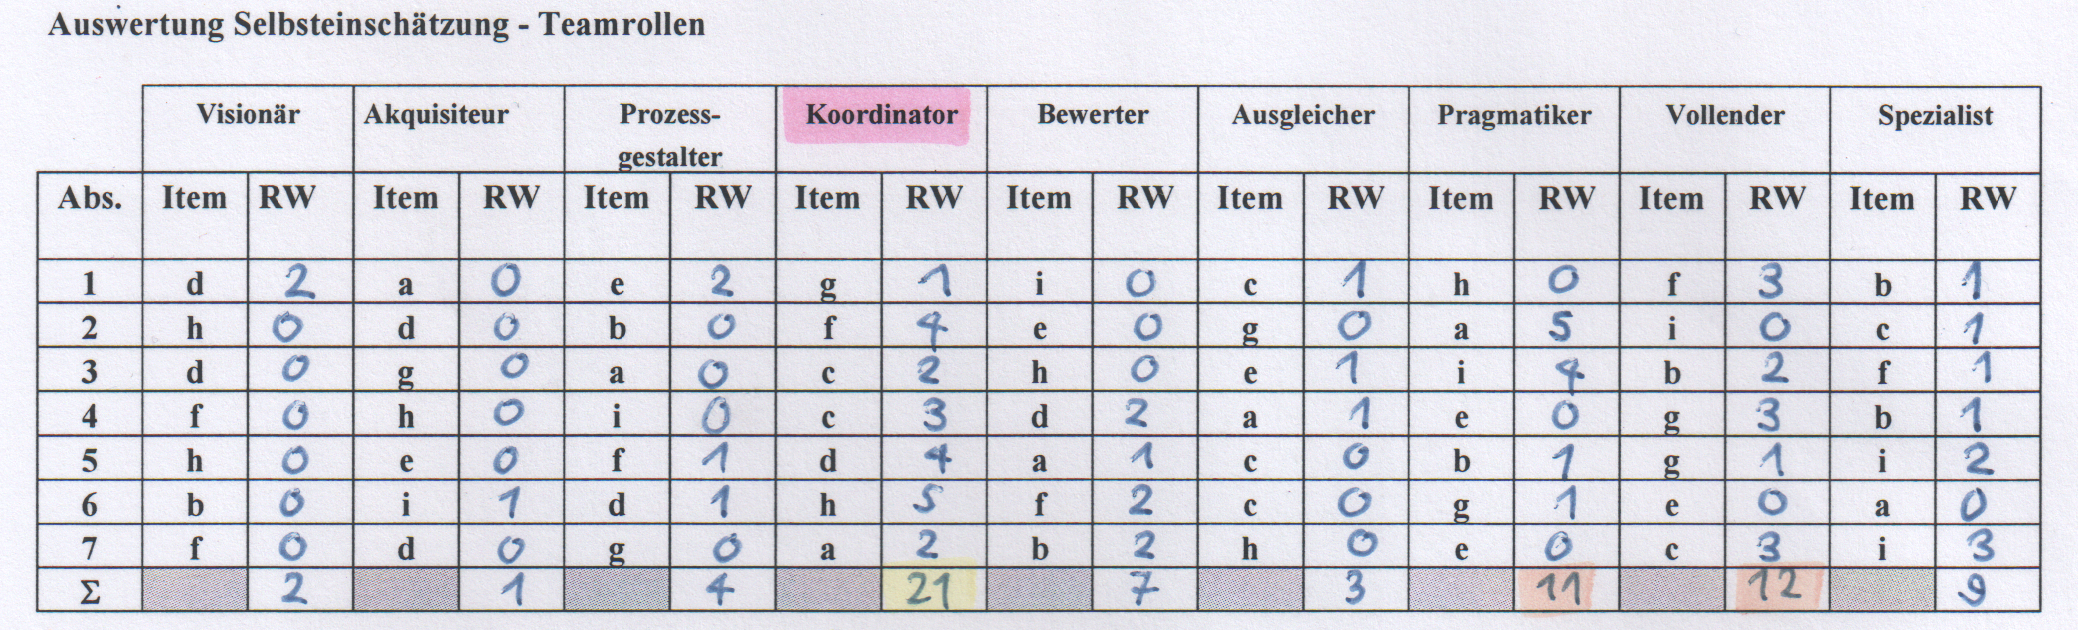
\includegraphics[height=39mm]{images/SelbsteinschaetzungHorat.png}

Tatsächlich erreichte, wie von mir im vornherein erwartet, die Rolle des Koordinators die höchste Punktzahl. Allerdings war ich überrascht mit welcher Deutlichkeit das Resultat ausfiel. Wie in obiger Grafik ersichtlich, haben die Rolle des Pragmatikers und des Vollenders die zweitgrösste Ausprägung (orange markiert). Auch sieht man, das die Visionärsrolle und die des Akquisiteurs fast keine Punkte erhalten haben. Die äusserst niedrige Punkteausbeute beim Visionär hat mich eher überrascht. Ich finde nämlich, das oft alternative Ansätze und neue Ideen von meiner Seite kommen.

\subsection*{Steve Gerome Kamga}
Das Resultat meines eigenen Lernprozesses nach der Belbin-Methode hat folgende Teamrollen gezeigt, die zu meiner Fähigkeiten, 
meinem Verhalten bei

\subsection*{Gökhan Kaya}

Meine Auswertung der Selbsteinschätzung gemäss Belbin ergab die folgende Punkteverteilung:

\begin{tabular}{lr}
  Visionär & 2 \\ 
  Akquisiteur & 5 \\ 
  Prozessgestalter & 8 \\ 
  Koordinator & 10 \\ 
  Bewerter & 2 \\
  Ausgleicher & 19 \\
  Pragmatiker & 7 \\
  Vollender & 6 \\
  Spezialist & \\
\end{tabular}
\newline


Somit ist zu sehen, dass folgende drei Teamrollen herausstechen:
%\renewcommand{\labelenumi}{\roman{enumi}} 
\begin{enumerate} 
\item Ausgleicher 
\item Spezialist
\item Koordinator
\end{enumerate}

Wobei besonders die Rolle des Ausgleichers mit 19 Punkten hervorsticht. Dies war für mich keine Überraschung, da sich während den Teamsitzungen bereits herauskristallisierte, dass der gute Teamzusammenhalt einer meiner Hauptziele geworden war. Ich habe mich entsprechend eingesetzt und immer wieder versucht herauszufinden, ob alle mit den getroffenen Entscheidungen zufrieden waren und wirklich nichts auszusetzen hatten. Falls doch habe ich versucht, mir die Meinung jedes einzelnen anzuhören und auszudiskutieren. 


\begin{comment}
\section{Lorem}
Lorem ipsum dolor sit amet, consectetur adipiscing elit. Sed gravida mollis placerat. Sed congue iaculis massa vitae dapibus. Fusce sed felis lorem. Suspendisse purus diam, sollicitudin vitae imperdiet ac, placerat eu metus. In luctus, metus vel dictum hendrerit, diam lacus cursus enim, eu porta augue lacus non metus. Pellentesque habitant morbi tristique senectus et netus et malesuada fames ac turpis egestas. Nullam nec orci eget metus pulvinar sagittis. Vestibulum ante ipsum primis in faucibus orci luctus et ultrices posuere cubilia Curae; Sed turpis lorem, aliquet eu ornare non, viverra ac urna.

Praesent libero lectus, ultrices eget pharetra sed, sollicitudin et est. Pellentesque quis urna eget lorem sodales venenatis eget nec quam. In sagittis aliquam auctor. Phasellus vitae ipsum purus, sit amet imperdiet nunc. Pellentesque habitant morbi tristique senectus et netus et malesuada fames ac turpis egestas. Ut malesuada nibh ut lectus scelerisque sed iaculis lectus varius. Nulla blandit turpis tortor. Nulla facilisi. Cum sociis natoque penatibus et magnis dis parturient montes, nascetur ridiculus mus. Nam leo ante, porta vel scelerisque at, volutpat eu sapien. Aliquam viverra adipiscing sapien et porta. Sed quis diam ut sem tincidunt consectetur varius non dolor. Fusce fermentum, quam vitae suscipit euismod, leo erat malesuada ante, ac consequat est lacus eget enim. Proin lacinia justo et est vehicula adipiscing rhoncus lacus mollis.	
\end{comment}